%% packages
\documentclass{article}
\usepackage[a4paper, left=2.0cm, right=2.0cm, top=3.5cm]{geometry}
\usepackage[ngerman]{babel}
\usepackage{graphicx}
\usepackage{multicol}
\usepackage{amssymb}
\usepackage{titlesec}
\usepackage{wrapfig}
\usepackage{blindtext}
\usepackage{lipsum}
\usepackage{caption}
\usepackage{listings}
\usepackage{fancyhdr}
\usepackage{nopageno}
\usepackage{authblk}
\usepackage{amsmath} % tons of math stuff
\usepackage{mathtools} % e.g. alignment within matrix
%\usepackage{bm} % provides shorthand for bold in math mode
\usepackage{dsfont} % \mathds makes double stroke digits
\usepackage{esdiff} % provides \diff
%\usepackage[ISO]{diffcoeff}
\usepackage{xcolor}
\usepackage{csquotes} % e.g. provides \enquote
\usepackage[separate-uncertainty=true]{siunitx} % units
\usepackage{xcolor} % colored text
\usepackage[l3]{csvsimple}
\usepackage{subcaption}
\usepackage{physics}
\usepackage{hyperref}
\usepackage{nameref}
\hypersetup{colorlinks=true, linkcolor=black, pdfhighlight={/N}}
\usepackage{tcolorbox}
\usepackage{amsthm}
\usepackage{gensymb} % add \degree in math mode?
\usepackage{newunicodechar} % define custom unicode characters




%\fancyhf[]{}

%% custom stuff
% own units
\DeclareSIUnit \VSS {\ensuremath{V_\mathrm{SS}}}
\DeclareSIUnit \VS {\ensuremath{V_\mathrm{S}}}
\DeclareSIUnit \Veff {\ensuremath{V_\mathrm{eff}}}
\DeclareSIUnit \Vpp {\ensuremath{V_\mathrm{pp}}}
\DeclareSIUnit \Vp {\ensuremath{V_\mathrm{p}}}
\DeclareSIUnit \VRMS {\ensuremath{V_\mathrm{RMS}}}
\DeclareSIUnit \ASS {\ensuremath{A_\mathrm{SS}}}
\DeclareSIUnit \AS {\ensuremath{A_\mathrm{S}}}
\DeclareSIUnit \Aeff {\ensuremath{A_\mathrm{eff}}}
\DeclareSIUnit \App {\ensuremath{A_\mathrm{pp}}}
\DeclareSIUnit \Ap {\ensuremath{A_\mathrm{p}}}
\DeclareSIUnit \ARMS {\ensuremath{A_\mathrm{RMS}}}

% change subsection numbering to capital letters
\newcommand{\subsectionAlph}{ \renewcommand{\thesubsection}{\arabic{section}.\Alph{subsection}} }
% change subsection numbering to lowercase letters
\newcommand{\subsectionalph}{ \renewcommand{\thesubsection}{\arabic{section}.\alph{subsection}} }
% change subsubsection numbering to lowercase letters
\newcommand{\subsubsectionalph}{ \renewcommand{\thesubsubsection}{\arabic{section}.\arabic{subsection}.\alph{subsubsection}} }
% own fig. that works with multicols
\newenvironment{Figure}
  {\par\medskip\noindent\minipage{\linewidth}}
  {\endminipage\par\medskip}
\newcommand*{\inputPath}{./plot} % prepend this command to the argument of all input commands
\graphicspath{ {./images/}{./figure/}{../plot/}{../../plot} }
% own enviroment for definitions
\newenvironment{definition}[1]
{\begin{quote} \noindent \textbf{\textit{#1\ifx&#1& \else : \fi}} \itshape}
{\end{quote}}

\newunicodechar{°}{\degree}


% own commands
% \newcommand{\rarr}{$\to\,$} %A$\,\to\,$B
\newcommand{\defc}{black}
\newcommand{\colorT}[2][blue]{\color{#1}{#2}\color{\defc}}
\newcommand{\redq}{\color{red}(?)\color{\defc}}
\newcommand{\question}[1]{\colorT[purple]{\textbf{(#1)}}}
\newcommand{\todo}[1]{\colorT[red]{\textbf{(#1)}}}
\newcommand{\mr}{\mathrm}

%% preparation
\begin{titlepage}
    \title{Praktikum Atome, Moleküle, kondensierte Materie \\ Versuch 402: Quantelung von Energie}
    \author[1]{Carlos Pascua\thanks{s87cpasc@uni-bonn.de}}
    \author[1]{Michael Vogt\thanks{s65mvogt@uni-bonn.de}}
    \affil[1]{Uni Bonn}
    %\date{\today}
\end{titlepage}


%% document
\begin{document}

\pagenumbering{gobble}
\maketitle
\tableofcontents
\newpage
\pagenumbering{arabic}

\pagestyle{fancy}
\fancyhead[R]{\thepage}
\fancyhead[L]{\leftmark}

\section*{Einleitung}


\section{Teil l: Bestimmung des Planckschen Wirkungsquantum}

\section{Balmer-Serie}
Es soll anhand einer Balmer-Lampe die Balmer-Serie von Spektrallinien des Wasserstoffs beobachtet und aus den Ergebnissen
die Rydberg-Konstante sowie das Plank'sche Wirkungsquantum bestimmt werden. Außerdem wird die Isotopieaufspaltung zwischen Wasserstoff und Deuterium quantifiziert.

Als Balmer-Serie bezeichnet man eine bestimmte Reihe von Spektrallinien des Wasserstoffatoms, die besonders gut mit dem bloßen Auge zu sehen sind
und 1885 von Johann Jakob Balmer untersucht wurden \cite[S. 99]{demtröder3}. Das Vorhandensein diskreter Linien ist ein bedeutendes Beispiel der Quantelung von Energie.
Balmer fand empirisch eine Gleichung für die inverse Wellenlänge, welche einem Spezialfall der Rydberg-Formel
\begin{equation}
  \frac{1}{\lambda} = R \left(\frac{1}{n^2} - \frac{1}{m^2}\right)\ \cite{demtröder3} \label{eq:rydberg-formel}
\end{equation}
mit $R$ der \textit{Rydberg-Konstante} und $n=2$ entspricht.

Dieser Zusammenhang konnte schließlich mit dem Bohrschen Atommodell erklärt werden, demzufolge Elektronen auf diskreten Bahnen um den Atomkern kreisen
und Licht einer bestimmten Wellenlänge aussenden, wenn sie von einer höheren auf eine tiefere Bahn übergehen.
Die Balmer-Serie entspricht in diesem Modell den Übergängen der Elektronen von der $m$-ten ($m>2$) Schale auf die zweite Schale.

Heute kann das Verhalten stattdessen mithilfe der Quantenmechanik beschrieben werden, welche ebenfalls diskrete Energieniveaus der Elektronen vorhersagt.
Die Rydberg-Konstante kann theoretisch berechnet werden und es gilt
\begin{equation}
  R = \frac{\mu e^4}{8c\epsilon_0 h^3}~\cite[S.101]{demtröder3} \label{eq:rydberg-konstante} 
\end{equation}
mit $\mu$ der reduzierten Masse von Elektron und Kern $\mu = \frac{m_e m_K}{m_e+m_K}$.
Der Wert von $R$ hängt also von der Masse des Kerns ab. Für verschiedene Isotope des Wasserstoffs sind Linien mit leicht unterschiedlichen Wellenlängen
zu erwarten, was als \textit{Isotopieaufspaltung} bezeichnet wird.

\subsection{Versuchsaufbau}
Der verwendete Aufbau ist in Abb. \ref{fig:balmer-aufbau} gezeigt.
\begin{figure}[h]
  \centering
  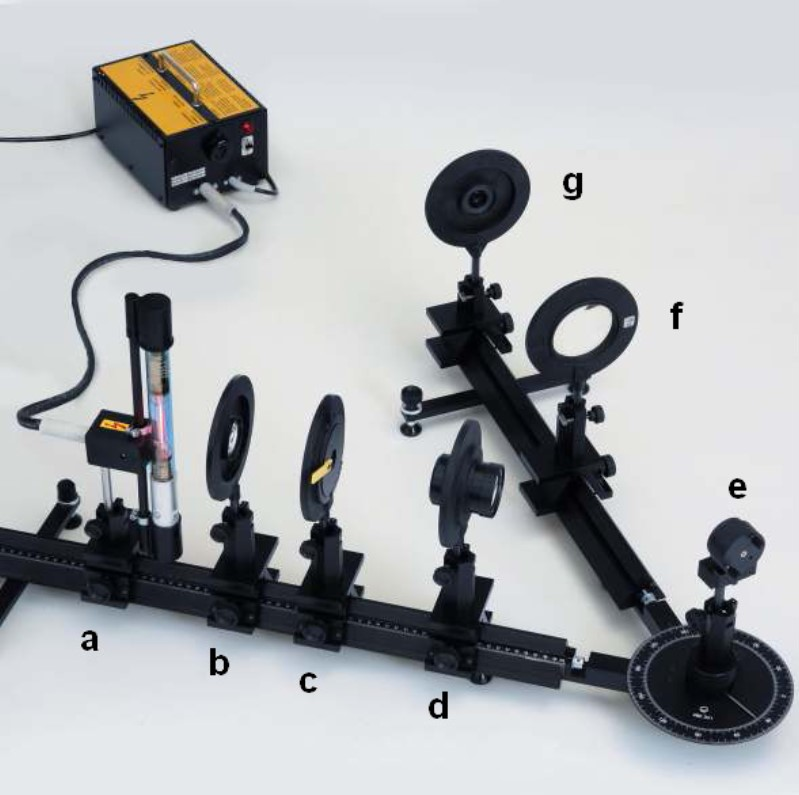
\includegraphics[width=0.5\textwidth]{balmer-aufbau}
  \caption{Aufbau zur Durchmessung der Balmer-Serie \cite{Anleitung}}
  \label{fig:balmer-aufbau}
\end{figure}
Die Linien sollen hier anhand einer Balmer-Lampe (a) beobachtet werden, welche herkömmliches sowie deuteriertes Wasser enthält.
Der Wasserdampf wird in der Lampe durch eine hohe Spannung zum Leuchten angeregt. Das Licht geht durch eine Linse (b), einen Spalt (c) 
und eine weitere Linse (d), welche als Projektionsobjektiv zur Kollimation dient, auf ein drehbar gelagertes Reflexionsgitter (e), welches hier als Interferometer dient. Das Muster kann an einer weiteren
drehbaren Schiene beobachtet werden, wo das Licht von einer weiteren Linse (f) auf das Okular (g) abgebildet wird.

Am Drehgelenk unter dem Gitter gibt es eine Winkelskala. Das Gitter wird zunächst auf \ang{0} gedreht und das Projektionsobjektiv in seinem Brennweitenabstand
(\SI{150}{\mm}, \cite{Anleitung}) hinter dem Spalt aufgestellt. Bei angeschalteter Lampe ist nun ein Bild des Spalts leicht neben dem Spalt zu sehen.
Damit das Gitter genau justiert ist, wird es in seiner Aufhängung so gedreht, dass das Bild des Spalts im Spalt selbst liegt.

Das Gitter wird gedreht, bis am Okular eine Linie sichtbar wird. Diese kann durch verschieben der Linse vor dem Okular scharf gestellt werden.
Die relevanten Winkel sind in Abb. \ref{fig:balmer-winkel} gezeigt. Wir haben für alle Messungen $\omega_B = \ang{140}$ werwendet.
Der Winkel des Gitters $\omega_G$ wird verändert, um unterschiedliche Linien zu betrachen. Für die Winkel $\alpha$ und $\beta$, welche
direkte Relevanz für die Gittergleichung haben, ergeben sich dann durch
\begin{align}
  \alpha &= \omega_G \nonumber \\
  \beta &= \ang{180} + \omega_G - \omega_B \label{eq:balmer-winkel}
\end{align}
Die Gittergleichung für konstruktive Interferenz lautet
\begin{equation}
  k\lambda = g(\sin(\alpha) + \sin(\beta)) \label{eq:gittergleichung}\ \cite{leybold-balmer}
\end{equation}
wobei hier immer die erste Ordnung mit $k=1$ beobachtet wird. $g$ ist die sogenannte Gitterkonstante,
die experimentell anhand des bekannten Spektrums von Quecksilber bestimmt werden soll.

\begin{figure}{h}
  \centering
  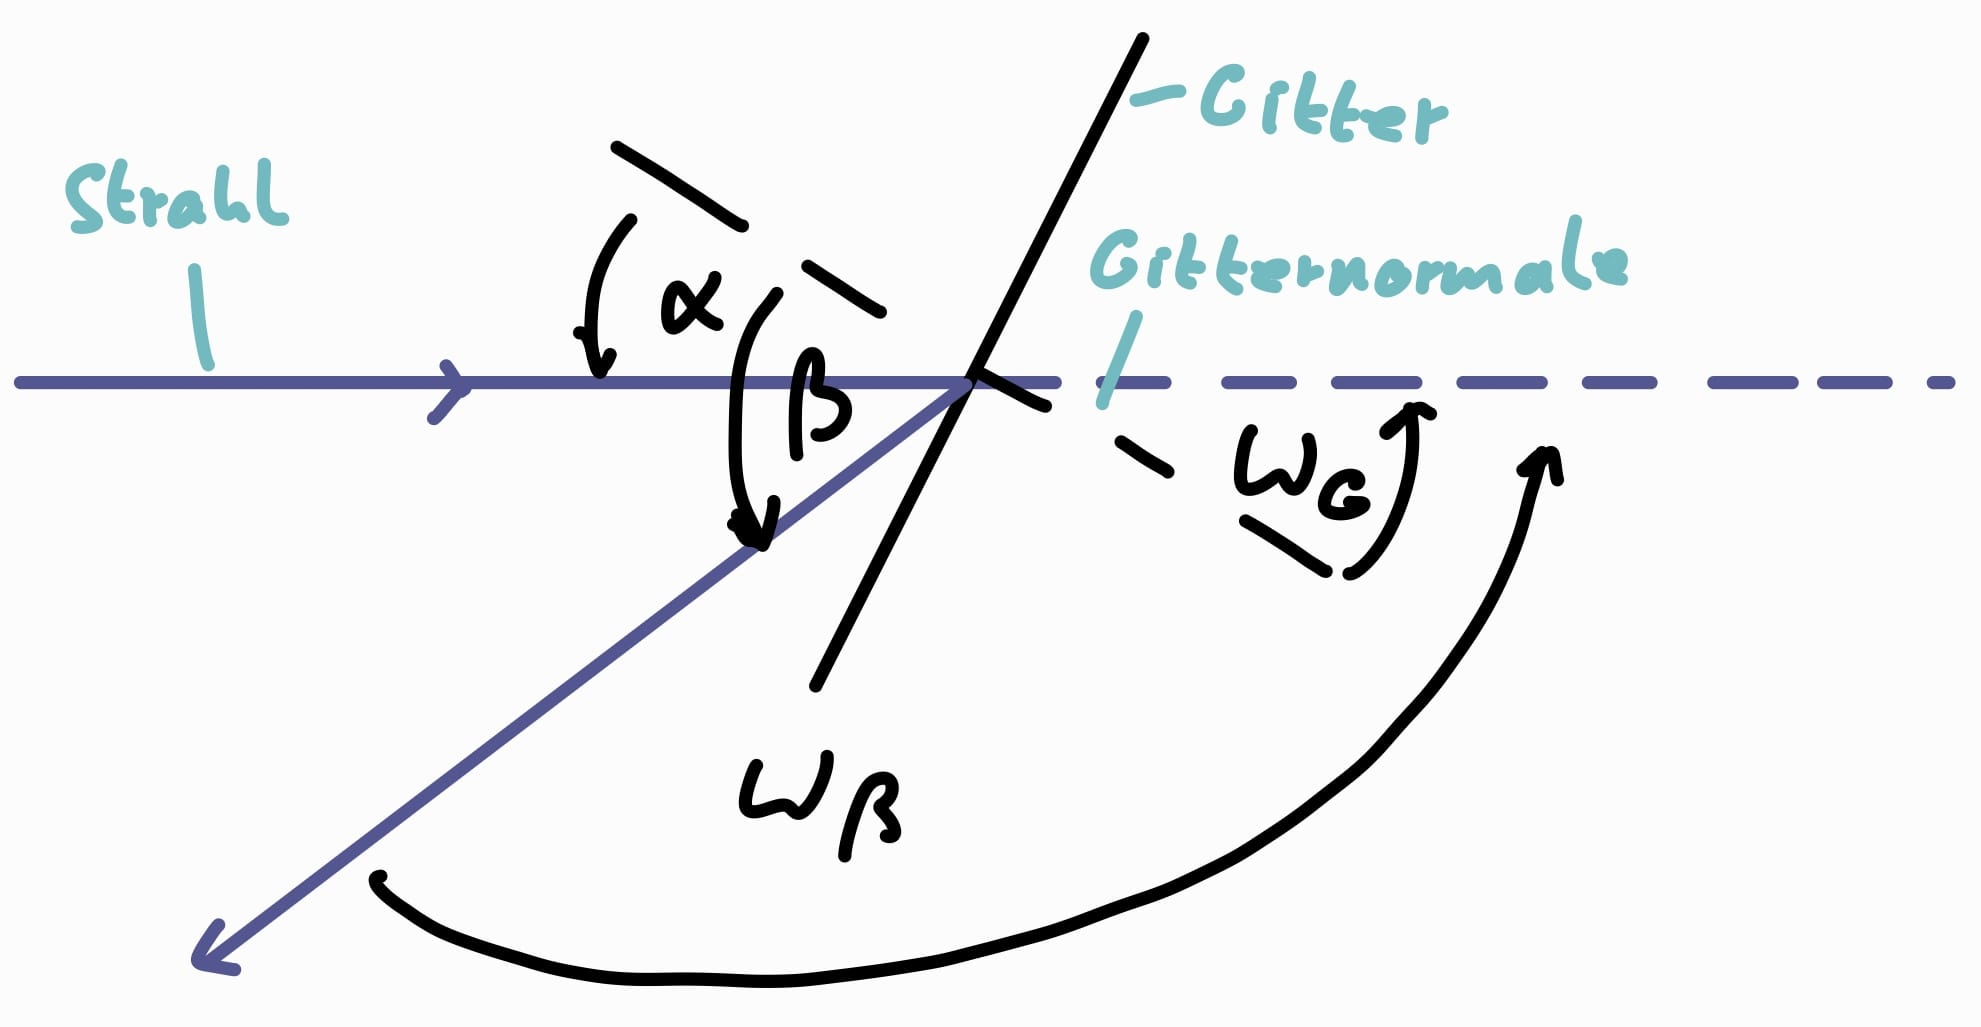
\includegraphics[width=0.5\textwidth]{balmer-winkel}
  \caption{Winkel bei der Messung der Balmer-Serie.}
  \label{fig:balmer-winkel}
\end{figure}

Das Okular hat außerdem eine Strichskala, welche dazu dient, kleine Winkelunterschiede zu messen und
hier für die Bestimmung der Isotopieaufspaltung verwendet werden kann.
% Das Zentrum der Skala liegt bei \SI{5}{\mm} und
Der Winkelunterschied zwischen zwei Linien bei $d_1$ und $d_2$ auf der Skala ergibt sich aus dem Abstand zur Abbildungslinse:
\begin{equation}
  \delta \beta = \tan^{-1}\left(\frac{\lvert d_2-d_1 \rvert}{f}\right) = \left\lvert \frac{d_2-d_1}{f} \right\rvert \label{eq:}
\end{equation}
wobei im zweiten Schritt die Kleinwinkelnäherung verwendet wurde und $f=\SI{300}{\mm}$ die Brennweite der Linse ist \cite{Anleitung}.

\subsection{Bestimmung der Gitterkonstanten}
Zunächst soll die Gitterkonstante $g$ des verwendeten Gitters bestimmt werden.
Hierzu sollen die Winkel verschiedener Hg-Linien gemessen und mit den bekannten Linien verglichen werden (Tab. \ref{tab:hg-linien}).
Zunächst wird also die Balmer-Lampe durch eine Hg-Spektrallampe ersetzt.
\begin{table}
  \centering
  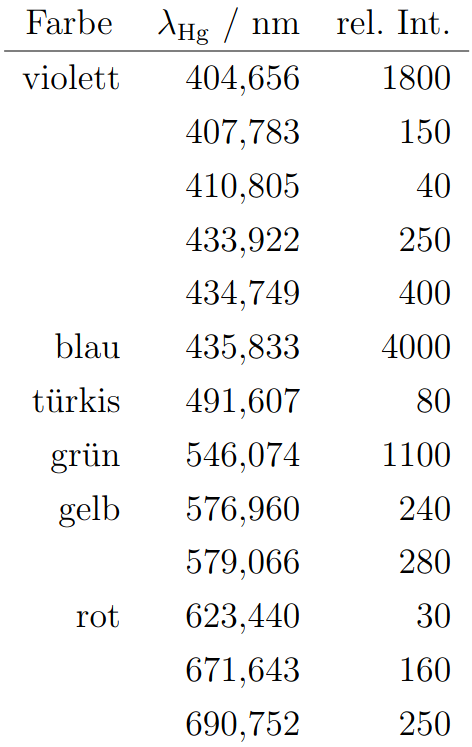
\includegraphics[width=0.2\textwidth]{hg-linien}
  \caption{Wellenlängen, Farben und Intensitäten des Hg-Spektrums. \cite{Anleitung}}
  \label{tab:hg-linien}
\end{table}

Die Winkel der beobachteten Linien zusammen mit der Farbe und der beobachteten Intensität (grobe Skala von $1$ bis $5$)
sind in Tab. \ref{tab:hg-beobachtung} gezeigt. Die Wellenlänge wurde anhand dieser Daten und Tab. \ref{tab:hg-linien} zugeordnet.
\begin{table}
  \caption{Beobachtete Daten und deren Auswertung für die Linien der Hg-Spektrallampe.
  Der Fehler der Winkel wird auf \ang{0.6} geschätzt.}
  \label{tab:hg-beobachtung}
\end{table}

$\alpha$ und $\beta$ wurden anhand von \eqref{eq:balmer-winkel} berechnet und aus der Gittergleichung \eqref{eq:gittergleichung} folgt
\[
  g = \frac{\lambda}{\sin(\alpha)+\sin(\beta)}
\]
Der Fehler von g wurde mit Gauß'scher Fehlerfortpflanzung berechnet.

Für die roten Linien erhalten wir stark von den anderen Messungen abweichende Gitterkonstanten.
Womöglich haben wir hier die Wellenlängen falsch zugeordnet und sie werden für die weitere Auswertung nicht verwendet.
Um aus den restlichen Messungen einen einzelnen Wert der Gitterkonstante zu erhalten, passen wir eine Gerade
an die Gittergleichung an (Abb. \ref{fig:fit-gitterkonstante}).
\begin{figure}{h}
  \centering
  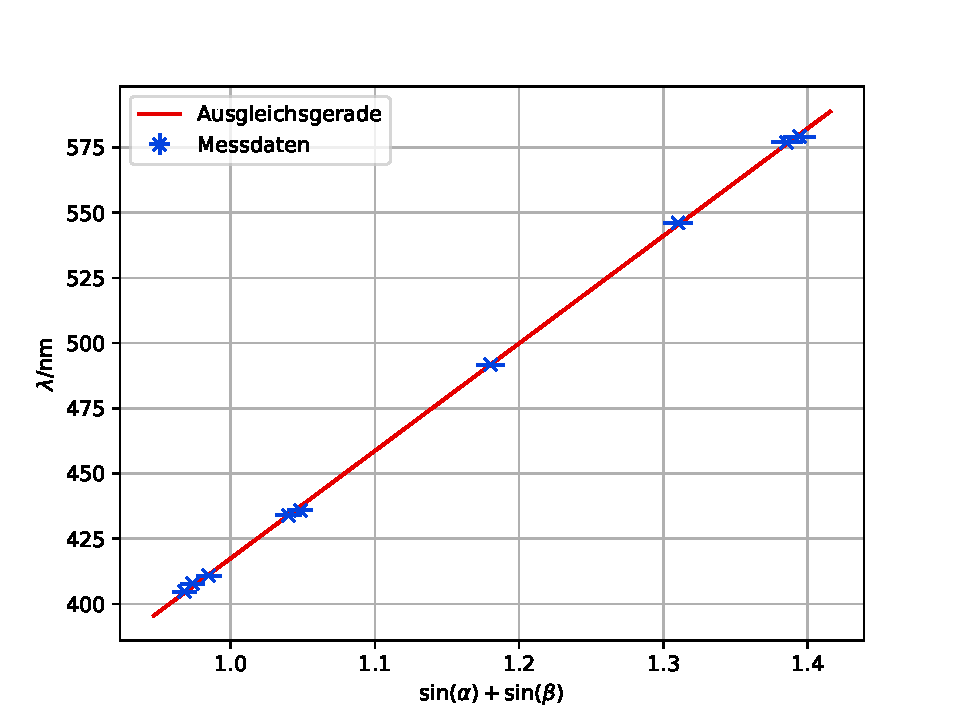
\includegraphics[width=0.5\textwidth]{fit-gitterkonstante}
  \caption{Linearer Fit zur Bestimmung der Gitterkonstante.}
  \label{fig:fit-gitterkonstante}
\end{figure}
Wir erhalten die Gleichung
\[
  \lambda = \dots + \frac{\dots}{\sin(\alpha)+\sin(\beta)} \todo{fill in}
\]
und damit
\[
  g = \dots \todo{fill in}
\]

Im Datenblatt \cite{leybold-balmer} ist angegeben,
dass das Gitter $\SI{2400}{\per\mm}$ Linien hat, was $g = \SI{416.67}{\nm}$ entspricht.
Die Abweichung von unserem Wert lässt sich dadurch erklären, dass das Gitter holographisch hergestellt wurde und
die Abstände bei solchen Verfahren nicht sehr genau sind \cite{Anleitung} \todo{stimmt das?}, was einer der Gründe ist,
warum wir die Gitterkonstante hier selbst experimentell bestimmt haben.


\subsection{Messung der Isotopieaufspaltung}
Auf zwei verschiedene Arten soll die Isotopieaufspaltung gemessen werden. Zunächst wird das Okular verwendet und anhand
der Position entlang der Strichskala die Aufspaltung zweier Linien bestimmt. Anschließend wir das Okular durch eine
CCD-Kamera ersetzt, deren Daten am Computer exportiert werden können.

Da die Aufspaltung der Wellenlänge $\delta \lambda$ zweier Linien nur klein ist, kann ihre Abhängigkeit von der
Winkelaufspaltung $\delta\beta$ linear genähert werden:
\begin{equation}
  \delta\lambda = \delta\beta \cdot \diffp{\lambda}{\beta} = g\cos(\beta)\delta\beta \label{eq:balmer-aufspaltung}
\end{equation}

\subsubsection{Messung mit Okular}
Die beobachteten Linien und ihre Positionen entlang der Strichskala des Okulars sind in Tab. \ref{tab:balmer-linien-okular}
gezeigt. Die Mitte der Strichskala liegt bei $d = \SI{5}{\mm}$.
\begin{table}[h]
  \centering
  % \csvsimple{../balmer_H.csv}
  % \csvsimple[
  %   head=true,
  %   separator=comma,
  % ]
  \csvautotabular{../balmer_H.csv}
  \caption{Messung der Balmer-Linien mit einem Okular, mit zugeordneter Quantenzahl $m$.}
  \label{tab:balmer-linien-okular}
\end{table}
% \begin{table}[h!]
%     \centering
%     % \csvsimple[
%     %     head=true,  % Use the first row as the table header
%     %     separator=comma,  % Specify the delimiter (comma is default)
%     %     tabular=|c|c|c|,  % Table format
%     %     table head=\hline Column 1 & Column 2 & Column 3 \\ \hline,
%     %     late after line=\\\hline  % Line after each row
%     % ]{example.csv}
% \end{table}



\clearpage
\section{Fazit}


\clearpage
\begin{thebibliography}{9}

\bibitem{Anleitung}
\textit{Physikalisches Praktikum Teil IV -- Versuchsbeschreibungen}, Universität Bonn, 10.10.2024

\bibitem{demtröder3}
\textit{Experimentalphysik 3 -- Atome, Moleküle, Festkörper}, 5. Auflage, Wolfgang Demtröder, 2016

\bibitem{leybold-balmer}
\textit{Balmer-Serie des Wasserstoff}, Leybold Didactic, Abruf 17.11.2024

\end{thebibliography}

\end{document}

